\documentclass{project-logbook}

\usepackage{csquotes}
\usepackage{lastpage}
% You can add the maintainer and the contributors in the preamble of the document

% This is how you add the maintainer (there is only one) the maintainer is automatically a contributor, the format is
% name, id (to appear in short messages), the affiliation.
\SetMaintainer{Jeffrey Liang}{u7013004}{ANU School of Computing}

% This is how you add a contributor, you can have as many contributors as you like (althought
% there is a limited space on the front page, at least 25 contributors fit in the front page, which should
% be more than enought).
% The format is similar to Maintainer: key, name, id, affiliation. The key field is the difference. It is used
% to internally identify the contributor, such that one can access the data of each contributor. This is discussed
% below.


% The same goes for the titles of the project.
% Three levels can be used. The project title sets the main title of the project, which appears in the middle of the front page.
% The project subtitle appears below the project title in the front page and serves as additional information to the title.
%  Additionally, a shorter title must be set to appear on the header of the document, the header name.
\SetProjectTitle{Honours Logbook}
\SetProjectSubtitle{The subtitle of the project}
\SetProjectHeaderName{The very fancy project}

% Below the project there is space to add a brief summary of the project for easy understanding when looking at the front page.
\SetProjectSummary{Here you can add a brief summary of your project such that someone can quickly see what it is about, do not spend more than two lines on it.}

% The institution logo (typically the one of the maintainer, but a logo file combining different logos can be used, but needs to
% be in one single pdf or png file) can be set using the following macro
\SetInstitutionLogo{figures/mcod_logo.png}

% Set the bibliography file
\addbibresource{mybib.bib}

% Start the document
\begin{document}

%----------------------------------------------------------------------------------------
%  Front page
%----------------------------------------------------------------------------------------

% The front page is constructed like this, it simply adds the logo, title, subtitle, summary, the maintainer's information, along
% with the list of all contributors.
\MakeFrontPage

% Standard LaTeX can be used throughout the document, but custom functionality has been added for simplifying some recurrent tasks and
% ensuring a consistent format.


%----------------------------------------------------------------------------------------
%  Body of the document
%----------------------------------------------------------------------------------------
\newpage

% The document is separated into sections, which in turn can be subdivided into subsections
\section{Overview} \label{sec:overview}
	% Sections start in a new page, for this reason sections contain clearly disjoint parts of the document
	This document shows an example of how to use the \texttt{project-logbook} \LaTeX~class. This class is based upon the \texttt{article} class and may be used together with other packages for additional functionality. This class implements functionality for simplifying writing project/research logbooks and unifying its layout. We will  go over the different functionalities to display how to use them.

	\subsection{Preamble}
		In the preamble of the document you may set several parameters of this document.

		\subsubsection{Maintainer and contributors}
			Everyone who contributes to this document, should be added as a contributor. In this way it is know who contributed and we can also use this to identify who added some elements. Adding a contributor is done with \texttt{\textbackslash CreateContributor\string{<key>\string}\string{<name>\string}\string{<id>\string}\string{<affiliation>\string}}, where
			\begin{description}
				\item[\texttt{<key>}] is the shorthand used to internally identify a contributor and to retrieve its data, this should be a short word without special characters.
				\item[\texttt{<name>}] is the full name of the contributor to display on the front page (but may also be used in other situations if desired).
				\item[\texttt{<id>}] is the abbreviation of the contributor name, to display when associating the contributor to a note (see below) or a meeting minutes box (see below).
				\item[\texttt{<affiliation>}] is the affiliation of the contributor, mainly to display on the front page.
    			\end{description}

			This document is maintained by a unique maintainer, which is automatically defined as a contributor with key \texttt{maintainer}. The maintainer can be set in the preamble with  \texttt{\textbackslash SetMaintainer\string{<name>\string}\string{<id>\string}\string{<affiliation>\string}}. The meaning of the different input parameters is identical to what was seen above for the contributor.

			The maintainer name, id, and affiliation can be accessed via the commands \texttt{\textbackslash MaintainerName}, \texttt{\textbackslash Maintainerid} and \texttt{\textbackslash MaintainerInsitution}, which for this case gives: \MaintainerName~(name), \Maintainerid~(id), and \MaintainerInstitution~(affiliation).

			In a similar way, a contributor can be accessed via the commands \texttt{\textbackslash ContributorName\string{<key>\string}}, \texttt{\textbackslash Contributorid\string{<key>\string}}, and \texttt{\textbackslash ContributorInstitution\string{<key>\string}}, which for this case gives (for key \texttt{chalmers}):  \ContributorName{chalmers}~(name), \Contributorid{chalmers}~(id), and \ContributorInstitution{chalmers}~(affiliation).

		\subsubsection{Project title, subtitle, and header name}
			The project title (which appears in the center of the front page) can be set in the preamble of the document with \texttt{\textbackslash SetProjectTitle\string{<title>\string}}, where \texttt{<title>} is the title we wish to set.

			Below the project title we can have a project subtitle, which can also be set in the preamble of the document with \texttt{\textbackslash SetProjectSubtitle\string{<subtitle>\string}}, where \texttt{<subtitle>} is the subtitle we wish to set.

		\subsubsection{Maintainer institution logo}
			On the top right corner of the front page you can add the logo of the institution of the maintainer. This can be done in the preamble with the command \texttt{\textbackslash SetInstitutionLogo\string{<path\_to\_file>\string}}, where \texttt{<path\_to\_file>} is the path to a .pdf or .png file. If you do not want to show a logo, use a white figure.

	\subsection{Body}
		The front page is generated with the command \texttt{\textbackslash MakeFrontPage}. This automatically adds the table of contents on the second page of the document, with direct links to the sections, for quick access.

		One important section is the Meetings section, which is subdivided into External and Internal. The External subsection contains the minutes of the meetings with external partners and the Internal sections contains the internal meetings associated to the institution of the Maintainer. Any contributor (including the maintainer) can be an author of Meeting minutes.

		Following the Meetings section, any number of sections can be added focussing on specific topics. The goal of these is to discuss the current state of the development of a particular part of the project. More discussed below.

		Following these sections, there is an Appendix, containing the list of references (papers to use as reference later when writing a paper), a list of resources such as a link to a video presentation, a tutorial, or something else that is less formal than a reference. In the end, you have a list of TODOs that have been defined in the document. They appear in the order in which they appeared in the document, not by writing date.


\section{Progress Logbook}
	\subsection{Progress}
	\begin{MeetingMinutes}{Sun 12/05/2024}{u7013004}
		Reading MeshSDF paper.
	\end{MeetingMinutes}
	
	\begin{MeetingMinutes}{Sat 18/05/2024}{u7013004}
		Reading MeshSDF, the Learning Implicit Fields papers, and Structure from Motion. Need to look up what the following mean:
		\begin{itemize}
			\item differentiable rendering, surface reconstruction
		\end{itemize}
	\end{MeetingMinutes}
	
	\begin{MeetingMinutes}{Sun 19/05/2024}{u7013004}
		Reading more from Structure-from-Motion Revisited. Didn't really understand much of SfM last night.
	\end{MeetingMinutes}
	
	\begin{MeetingMinutes}{Thu 27/06/2024}{u7013004}
		Attempting 3D version of the ellipse problem. \\
		Question: Why do we invert the $u_i$s? Answer: you bring the 1 over and multiply by some expression on both sides.
	\end{MeetingMinutes}
	
	\begin{MeetingMinutes}{Fri 5/07/2024}{u7013004}
		Having been making headway on the non-axis-aligned ellipsoid.
		I've been able to fit an ellipse to one but I haven't been able to do the bi-level optimisation.
		I'm going to try a couple approaches:
		\begin{itemize}
			\item reparametrise everything to radians and $a,b,c$ rather than squared inverses of semi-axes 
			\item try original objective function rather than focusing on optimising rotation 
			\item last resort is to figure out what the SqrtBackward error is
		\end{itemize}
	\end{MeetingMinutes}
	
	\begin{MeetingMinutes}{Sun 7/07/2024}{u7013004}
		Was able to switch implementation to radians and $a,b,c$ rather than squared inverses $1/a^2,...,1/c^2$. 
		It's still temperamental though and will hopefully be finetuned when meeting with Chamin who hopefully has a few tricks.
		Going to read some papers today about DRWR and the DDN and take notes to try and fully understand derivations etc.
	\end{MeetingMinutes}
	
	\begin{MeetingMinutes}{Sat 20/07/2024}{u7013004}
		Reading additional papers and waiting for Steve's meeting. Reading "Small Steps and Level Sets" by Chamin and will document.
	\end{MeetingMinutes}

	\begin{MeetingMinutes}{Mon 29/07/2024}{u7013004}
		Trying to do experiments to ensure I know the cause of my errors and that it's not some implementation error.
		Will do:
		\begin{itemize}
			\item small volume initialisations
			\item close to ground truth initialisations
			\item tightening the constraint slowly
			\item PCA?
		\end{itemize} 
		Ideal semi-axes lengths is: 0.28209
		Trials:
		\begin{enumerate}
			\item initialisation: 0.2, 0.4, 0.3, 30°, 25°, -120°. final: 0.271, 0.296,0.28, 29.98°, 24.99°, 60.0°
			\item initialisation: 0.1, 0.2, 0.3, 30°, 25°, -120°. final: 0.479, 0.29,0.0913, 83.83°, 128.2°, 47.02° (no improvement).
				 \\ the issue here is that the fitted ellipse is too far away from a sphere for it to approach a sphere?
			\item initialisation: close to ideal. result: optimised fine and as expected.
		\end{enumerate}
		Perhaps farthest point sampling would prevent the ellipse from over concentrating at the poles.

		Issue! For Trial 2, a close reinitialisation of 0.1, 0.3, 0.5 and angles 30°, 25°, -120° worked well. In fact, an exact reinitialisation worked?! But then when reverting back so that the fitted ellipse had those params, the gradients calculated were zero.

		Steps to reproduce error:
		\begin{enumerate}
			\item Initialise with 0.1, 0.2, 0.3 and 30°, 25°, -120°. Run the first cell and then second cell, and we should see no deformation of the fitted ellipsoid to a sphere - the parameters remain as 0.479, 0.29,0.0913, 83.83°, 128.2°, 47.02°. The gradients are very close to 0.
			\item Initialise with the parameters 0.479, 0.29,0.0913 and 83.83°, 128.2°, 47.02°. We see that the gradients are non-zero and we optimise to a sphere.
		\end{enumerate}
		a, b, c = 0.4786546028, 0.2901328092,0.09132074619 \\ 
		yaw, pitch, roll = 83.82856741, 128.3492915, 47.0228292

	\end{MeetingMinutes}

\section{Topic A to focus on} \label{sec:topic_A}
	We can use sections organize the text into different parts  such that specific topics are addressed in their own section.

	\begin{HighlightedNote}{}
		Sections always start at the top of a new page in order to generate clearly separated parts of the document. In this first section (Overview) one should introduce what this project is about, in a high level so you can do a simple explanation of the topic and the research challenges, who is involved, etc.

		Since this information is important, we have added it within a \texttt{HighlightedNote} environment. This is the version without a title.
	\end{HighlightedNote}

	\begin{HighlightedNote}{You can add multiple things inside a \texttt{HighlightedNote}}
		And this is the version with a title. You can use the title for example if you want to clearly state what is is, or if you want to make a larger note and give an idea of what it is about.

		You can add equations to clarify your ideas
		\begin{equation}
			e^{i\pi} + 1 = 0
		\end{equation}

		Some tables

		\begin{center}
			\begin{tabular}{ccccc}
            			{}  & \multicolumn{1}{c}{$A$} & \multicolumn{1}{c}{$N$} & \multicolumn{1}{c}{$S$} & \multicolumn{1}{c}{$A/S$} \\
            			\midrule
            			a & 292 & 117   & 409   & 0.714 \\
            			b & 104 & 386   & 490   & 0.212 \\
            			c & 24  & 7     & 31    & 0.774 \\
            			d & 28  & 27    & 55    & 0.509 \\
            			e & 183 & 1958  & 2141  & 0.085 \\
            			\midrule
            			& 631 & 2495 & 3126 & 0.202 \\
        			\end{tabular}
    		\end{center}
		and other elements.

	\end{HighlightedNote}

	\begin{HighlightedNote}{With a fancy title}
		The \texttt{HighlightedNotes} environment that generates these fancy boxes, can be used with a title \texttt{\textbackslash begin\string{HighlightedNotes\string}\string{the\_title\_text\string}}, as in this case, or without a title \texttt{\textbackslash begin\string{HighlightedNotes\string}\string{\string}}, as in the previous case.
	\end{HighlightedNote}

	\subsection{A subsection}
		You can subdivide your section in a finer level using \texttt{\textbackslash subsection}.

		\subsubsection{A subsubsection}
			The subsections can be subdivided with \texttt{\textbackslash subsubsection}.

			\subsubsubsection{A subsubsubsection}
				And an additional level was added to subdivide subsubsections named \texttt{\textbackslash subsubsubsection}. This should give more than enough subdivision levels to your text for fine grained organisation.

				\begin{HighlightedNote}{}
					In most Machine Learning research projects you will be using some kind of samples from a Dataset to learn a model. Thus it is extremely important that you carefully describe the dataset and why you believe is a good dataset for the project and what type of preprocessing are you going to apply.
				\end{HighlightedNote}

				As usual, you can use your references to cite relevant articles as \cite{einstein} and \cite{knuth-fa}.

				You can use tables and, of course, make references to them, like the amazing \tabref{tab:populations}.


				\begin{table}[ht]
					\centering
						\begin{subtable}{0.48\textwidth}
							\centering
        								\begin{tabular}{*{5}{r}}
									{}  & \multicolumn{1}{c}{$A$} & \multicolumn{1}{c}{$N$} & \multicolumn{1}{c}{$S$} & \multicolumn{1}{c}{$A/S$} \\
									\midrule
									a & 292 & 117   & 409   & 0.714 \\
									b & 104 & 386   & 490   & 0.212 \\
									c & 24  & 7     & 31    & 0.774 \\
									d & 28  & 27    & 55    & 0.509 \\
									e & 183 & 1958  & 2141  & 0.085 \\
									\midrule
									& 631 & 2495 & 3126 & 0.202 \\
								\end{tabular}
							\caption{Training Set}
						\end{subtable}
    						%
    						\begin{subtable}{0.48\textwidth}
        							\centering
        								\begin{tabular}{*{6}{r}}
									{}  & \multicolumn{1}{c}{$A'$} & \multicolumn{1}{c}{$N'$} & \multicolumn{1}{c}{$S'$} & \multicolumn{1}{c}{$A'/S'$} & $S'/S$ \\
									\midrule
									a & 40  & 40    & 80    & 0.5   & 0.20 \\
									b & 49  & 49    & 98    & 0.5   & 0.20 \\
									c & 4   & 3     & 7     & 0.57  & 0.23 \\
									d & 5   & 5     & 10    & 0.5   & 0.18 \\
									e & 53  & 53    & 106   & 0.5   & 0.05 \\
									\midrule
									& 151 & 150 & 301 & 0.50 & 0.10 \\
								\end{tabular}
								\caption{Validation Set}
						\end{subtable}

    						\caption{Population properties $A \equiv$ Abnormal, $N\equiv$ Normal, $S\equiv A+N$}
    						\label{tab:populations}
				\end{table}

	\subsection{Another subsection} \label{sub:another_subsection}
		Relevant equations can be added

		\begin{equation}
    			x_i' \gets \frac{x_i-\bar{x}}{\upsigma}
		\end{equation}
		\begin{equation}
    			\bar{x} = \frac{1}{N}\sum_{i=1}^{N} x_i \qquad \upsigma^2 = {\frac{1}{N}\sum_{i=1}^{N} (x_i-\bar{x})}
		\end{equation}

		\begin{HighlightedNote}{Strike-through}
 			Often you will be wrong on your assumptions, but do not throw them away completely, just cross them out in case you need them later using the \texttt{\textbackslash sout} command and it will look like \sout{this} or \texttt{\textbackslash soutthick} command and it will look like \soutthick{this}
		\end{HighlightedNote}

		\sout{Medoid computation is perfomed at $f_s'' = f_s'/5 = \SI{200}{\kilo\hertz}$ to speed computation. Simple analysis was performed to check that the features extracted from these 200Hz-medoids were approximately the same as the ones extracted from the  1khz-medoids.}

		\soutthick{Downsampling can be seen as a problem of information loss in the frequency spectrum. If the frequency content $f > f_s/(2N)$ is mostly empty for $N$ when we downsample by said $N$ we will only be losing information in that range.}

		\begin{HighlightedNote}{TODOs}
			You will often have pending tasks that you need to track. This project logbook allows you to include both high and low priority todos that will be summarised in a list at the end of the file. Use the commands \texttt{\textbackslash hightodo\string{<date\_added>\string}\string{<author\_key>\string}} and \texttt{\textbackslash lowtodo}, including a date is recommended for tracking purposes.

			Note: define your \texttt{userId} in the preamble
		\end{HighlightedNote}


		\lowtodo{2016-05-23}{chalmers}{Try the code in the newest version of numpy compiled with optimized BLAS.}

		\hightodo{2016-05-27}{maintainer}{Perform convergence analysis with the latest version of the code.}


\section{Topic B to focus on} \label{sec:topic_B}

	\subsection{Algorithms} \label{sub:algorithms}

		\begin{HighlightedNote}{}
			Sometimes the most straightforward way to explain a procedure is just to give it in a algorithmic format, it takes a little time but it will force you to go through the steps and you will most likely be able to reuse it on you paper. For the full documentation see here \url{https://texdoc.org/serve/algorithmicx/0}.
		\end{HighlightedNote}

		\begin{algorithm}
			\caption{Euclid’s algorithm}\label{alg:euclid}
			\begin{algorithmic}[1]
				\Procedure{Euclid}{$a,b$}\Comment{The g.c.d. of a and b}
					\State $r\gets a\bmod b$
					\While{$r\not=0$}\Comment{We have the answer if r is 0}
						\State $a\gets b$
						\State $b\gets r$
						\State $r\gets a\bmod b$
					\EndWhile\label{euclidendwhile}
					\State \textbf{return} $b$\Comment{The gcd is b}
				\EndProcedure
			\end{algorithmic}
		\end{algorithm}


	\subsection{Code} \label{sub:code}
		\begin{HighlightedNote}{}
			If the algorithm is too vague and you feel like you need the source code you can also insert it. You can put LaTeX code inside by using \texttt{<@ @>} delimiters, highlight small pieces of the code with \texttt{<| |>} delimiters, and highlight full lines (see the source code). For now only Python colored syntax highlighting is available, but most languages are supported and the color scheme can be added. More information available here \url{https://www.overleaf.com/learn/latex/Code_listing}.

			Note that these pieces of code in the \LaTeX~document must start with no indent.
		\end{HighlightedNote}

\begin{lstlisting}[style=Python, linebackgroundcolor={
	\ifnum \value{lstnumber}=8 \color{orange!30} \fi
	\ifnum \value{lstnumber}=10 \color{orange!30} \fi
	\ifnum \value{lstnumber}=17 \color{orange!30}\fi
	\ifnum \value{lstnumber}=18 \color{orange!30}\fi}]
def DTW_distance(s1, s2):
	"""
	Function to compute the Dynamic Time Warping in Python between two signals
	"""
	DTW={}

	for i in range(len(s1)):
		DTW[(i, -1)] = float('inf') # By default <@\color{pgreen} $\infty$@>
	for i in range(len(s2)):
		DTW[(-1, i)] = float('inf') # By default <@\color{pgreen} $\infty$@>
	DTW[(-1, -1)] = 0

	for i in range(len(s1)):
		for j in range(len(s2)):
			dist= <|(s1[i]-s2[j])**2|>
			DTW[(i,j)] = dist + min(DTW[(i-1, j)],DTW[(i, j-1)], \
				DTW[(i-1, j-1)])

	return sqrt(DTW[len(s1)-1, len(s2)-1])
\end{lstlisting}

	\subsection{Diagrams} \label{sub:diagrams}
		\begin{HighlightedNote}{}
			For simple diagrams I highly recommend learning TiKZ, you will be drawing the diagrams in pure \LaTeX which has a steep learning curve but once you get used to it, it can be quite easy to display and do \texttt{for} loops to draw multiples line at once.
		\end{HighlightedNote}

		\begin{figure}[!h]
			\centering
				\tikzset{%
  					every neuron/.style={
    						circle,
    						draw,
    						minimum size=1cm
  					},
  					neuron missing/.style={
    						draw=none,
    						scale=4,
    						text height=0.333cm,
    						execute at begin node=\color{black}$\vdots$
  					},
				}

				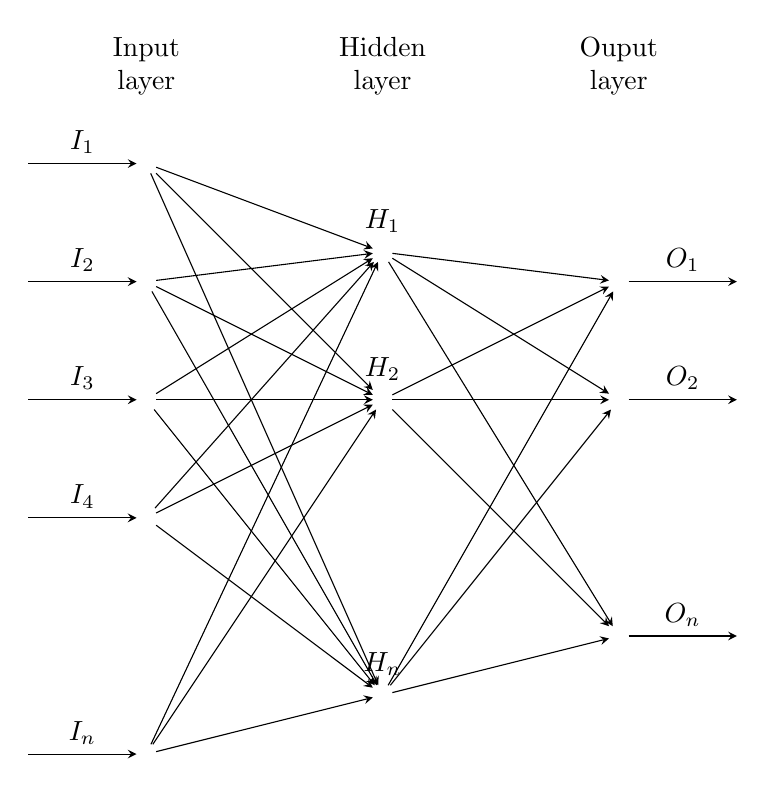
\begin{tikzpicture}[x=1.5cm, y=1.5cm, >=stealth]
					\foreach \m/\l [count=\y] in {1,2,3,4,missing,5}
  						\node [every neuron/.try, neuron \m/.try] (input-\m) at (0,2.5-\y) {};

					\foreach \m [count=\y] in {1,2,missing,3}
  						\node [every neuron/.try, neuron \m/.try ] (hidden-\m) at (2,2-\y*1.25) {};

					\foreach \m [count=\y] in {1,2,missing,3}
  						\node [every neuron/.try, neuron \m/.try ] (output-\m) at (4,1.5-\y) {};

					\foreach \l [count=\i] in {1,2,3,4,n}
  						\draw [<-] (input-\i) -- ++(-1,0)
    							node [above, midway] {$I_\l$};

					\foreach \l [count=\i] in {1,2,n}
  						\node [above] at (hidden-\i.north) {$H_\l$};

					\foreach \l [count=\i] in {1,2,n}
  						\draw [->] (output-\i) -- ++(1,0)
    							node [above, midway] {$O_\l$};

					\foreach \i in {1,...,5}
  						\foreach \j in {1,...,3}
    							\draw [->] (input-\i) -- (hidden-\j);

					\foreach \i in {1,...,3}
  						\foreach \j in {1,...,3}
    							\draw [->] (hidden-\i) -- (output-\j);

					\foreach \l [count=\x from 0] in {Input, Hidden, Ouput}
  						\node [align=center, above] at (\x*2,2) {\l \\ layer};

				\end{tikzpicture}
		\end{figure}

		\begin{HighlightedNote}{}
			However, sometimes you will need more complicated diagrams (or maybe you do not like TiKZ, in that case I recommend a vector drawing tool such as Inkscape which allows \LaTeX \,embedding)
		\end{HighlightedNote}

		% \begin{figure}[h]
    	% 		\includegraphics[width=0.9\textwidth]{figures/LSTM}
    	% 		\centering
    	% 		\caption{Gate Recurrent Unit in a Long Short Term Memory Neural Netwok (GRU-LSTM). \\ \emph{Credit to \url{https://colah.github.io/posts/2015-08-Understanding-LSTMs/}}}
    	% 		\label{fig:LSTM}
		% \end{figure}


\section{Topic C to focus on} \label{sec:topic_c}
	\subsection{Figures} \label{sub:figures}

		\begin{HighlightedNote}{}
			In general the best way to visualize your results will be some figures, I recommend Python's matplotlib for generating them or any other tool you are familiar with.
		\end{HighlightedNote}

		% \begin{figure}[htp]
    	% 		\centering
		% 		\begin{subfigure}{0.48\textwidth}
        % 					\centering
        % 						\includegraphics[width=\textwidth]{figures/sfem_1D_p3.pdf}
        % 						\caption{One-dimensional spectral element basis functions of polynomial degree $p = 3$ for subspace $G_{3} \subset H^{1}(\Omega)$, $\Omega\in\mathbb{R}$.}
    	% 			\end{subfigure}
    	% 			\hspace{.35cm}
    	% 			\begin{subfigure}{0.48\textwidth}
        % 					\centering
        % 						\includegraphics[width=\textwidth]{figures/sfem_1D_p5.pdf}
        % 						\caption{One-dimensional spectral element basis functions of polynomial degree $p = 5$ for the subspace $G_{5} \subset H^{1}(\Omega)$, $\Omega\in\mathbb{R}$.}
    	% 			\end{subfigure}

		% 		\vspace{1cm}

		% 		\begin{subfigure}{0.48\textwidth}
        % 					\centering
        % 						\includegraphics[width=\textwidth]{figures/sfem_p3.png}
        % 						\caption{Two-dimensional spectral element basis functions of polynomial degree $p = 3$ for subspace $G_{3} \subset H^{1}(\Omega)$, $\Omega\in\mathbb{R}^{2}$.}
    	% 			\end{subfigure}
    	% 			\hspace{.35cm}
    	% 			\begin{subfigure}{0.48\textwidth}
        % 					\centering
        % 						\includegraphics[width=\textwidth]{figures/sfem_p5.png}
        % 						\caption{Two-dimensional spectral element basis functions of polynomial degree $p = 5$ for the subspace $G_{5} \subset H^{1}(\Omega)$, $\Omega\in\mathbb{R}^{2}$.}
    	% 			\end{subfigure}

   		% 		\vspace{.25cm}
    	% 			\caption{Example basis functions for the spectral finite element method in 1D and 2D.}
    	% 			\label{fig:plots}
		% \end{figure}

% subsection figures (end)

\subsection{Tables} % (fold)
\label{sub:tables}

\begin{HighlightedNote}{}
\LaTeX \; booktab environments are really good to showcase and track your results, however they can get fairly messy. My suggestion is to generate them via Python automatically and store the results in either a plain text file or a spreadsheet (there are packages to read spreadsheets with Python)
\end{HighlightedNote}

\begin{table}[ht]
     \centering
     \begin{tabular}{rrrrrrrrrr}
         $\upsigma \setminus \tau$ & \multicolumn{1}{c}{0} &\multicolumn{1}{c}{1} &\multicolumn{1}{c}{2} &\multicolumn{1}{c}{3} &\multicolumn{1}{c}{4} &\multicolumn{1}{c}{5} &\multicolumn{1}{c}{6} &\multicolumn{1}{c}{7} &\multicolumn{1}{c}{8}\\
          \midrule
         0.0 & 100.0  &100.0  &100.0  &100.0  &100.0  &100.0  &100.0  &100.0  &100.0 \\
         0.2 & 100.0  &100.0  &100.0  &100.0  &100.0  &100.0  &100.0  &100.0  &100.0 \\
         0.4 & 100.0  &100.0  &100.0  &100.0  &100.0  &100.0  &100.0  &100.0  &100.0 \\
         0.6 & 98.6  &100.0  &100.0  &100.0  &100.0  &100.0  &100.0  &100.0  &100.0 \\
         0.8 & 84.7  &99.5  &100.0  &100.0  &100.0  &100.0  &100.0  &100.0  &100.0 \\
         1.0 & 28.1  &98.3  &99.9  &100.0  &100.0  &100.0  &100.0  &100.0  &100.0 \\
         1.2 & 1.3  &88.7  &99.4  &99.9  &99.8  &99.9  &100.0  &99.9  &100.0 \\
         1.4 & 0.0  &57.1  &96.2  &99.3  &99.0  &99.3  &99.4  &99.8  &99.7 \\
         1.6 & 0.0  &18.6  &81.2  &93.0  &93.7  &94.8  &95.6  &92.3  &93.3 \\
         1.8 & 0.0  &2.4  &42.8  &67.0  &70.1  &72.1  &69.0  &69.1  &68.6 \\
         2.0 & 0.0  &0.1  &9.0  &23.1  &24.5  &26.9  &28.2  &27.3  &27.3 \\
         \midrule
          $t$(ms) &27.92 &40.23 &77.30 &157.27 &252.05 &342.18 &381.46 &399.85 &413.72\\
     \end{tabular}
     \caption{Performance of the algorithm for 128-bit key and with multiple readings per key}
     \label{tab:error_128_avg}
 \end{table}

% subsection tables (end)

% section results (end)




%----------------------------------------------------------------------------------------
%   REFERENCE LIST
%----------------------------------------------------------------------------------------
\appendix

%% References (bibliography)
\section{References}
	\begin{HighlightedNote}{}
		Do not forget to cite the papers that you are using in your research, this way your work will be infinitely easier to write down and to review when the time comes.
	\end{HighlightedNote}

	% Add the bibliography without the header. You can remove the heading=none and \section{References} to have it in a different way.
	% Here we keep the references as a section from the Appendix, as an example
	\printbibliography[heading=none]


\section{Resources}
	\begin{HighlightedNote}{}
		It is a good idea to record sources that explain concepts or provide tools so the research is both better documented and if someone has to continue it there is enough supporting documentation.
	\end{HighlightedNote}
	\begin{itemize}
    		\item Quick read in DTW and Keogh Lower Bounding. \newline
			\url{http://alexminnaar.com/time-series-classification-and-clustering-with-python.html} \newline
			\url{http://nbviewer.jupyter.org/github/alexminnaar/time-series-classification-and-clustering/blob/master/Time%20Series%20Classification%20and%20Clustering.ipynb}

		\item Parallelizing DTW -- Good article on making a parallel version of DTW. Uses Keogh lower bound not as a linear approximation but as a pruning device. \newline
			\url{https://www.andrew.cmu.edu/user/mmohta/15418Project/finalreport.html}

    		\item Deep Learning
    			\begin{itemize}
        				\item Intro to LSTM \newline
					\url{https://colah.github.io/posts/2015-08-Understanding-LSTMs}
        				\item Intro to CNN \newline
					 \url{https://colah.github.io/posts/2014-07-Conv-Nets-Modular/}
				 \item Why are LSTMs are so useful, impressive result in character pattern and syntax learning \newline
					\url{https://karpathy.github.io/2015/05/21/rnn-effectiveness/}
    			\end{itemize}
	\end{itemize}


%% Add the list of todos in the end
\section{TODOS}
	\begin{HighlightedNote}{}
		Here you will have all your TODOs grouped with anchor links to the parts of the document where they are. Really handy if you do not know where to continue with your project.
	\end{HighlightedNote}

	\AddListOfTodos

\end{document}